\documentclass{article}
\usepackage[a4paper, top=2.5cm, bottom=2.5cm, left=2.5cm, right=2.5cm]{geometry}
\usepackage{graphicx}
\usepackage[utf8]{inputenc}
\usepackage{amsmath}
\usepackage{amsfonts}
\usepackage{float}
\usepackage{booktabs}
\usepackage{listings}

\title{\textbf{SDC2026 Midterm01 Report - Group 5}}
\author{
    Chang-Jyun Chen \\ \texttt{314605004} \and
    Ying-Pei Lin \\ \texttt{110611063}
}
\date{May 2026}

\begin{document}
\maketitle

\section{Introduction}
This report details the design and execution of our autonomous driving framework for the SDC2026 Midterm. The system integrates a robust LiDAR-based Simultaneous Localization and Mapping (SLAM) backend featuring advanced loop closure constraints, alongside a 3D Gaussian Splatting (3DGS) frontend optimized for outdoor cinematic reconstruction and geometric fidelity.

\section{Pipeline}

\subsection{LiDAR SLAM Module}
The LiDAR SLAM system processes consecutive point clouds to track vehicle ego-motion and construct a globally consistent map through a structured multi-step sequence:
\begin{enumerate}
    \item \textbf{Two-Stage ICP Alignment:} Every incoming scan (source) is registered against the active local submap (target) using a coarse-to-fine Generalized ICP (GICP) configuration to estimate the incremental odometry transformation $T \in SE(3)$.
    \item \textbf{Keyframe Registration:} If the frame meets the structural or kinematic tracking requirements, it is downsampled via a voxel filter and saved as a new keyframe within the \texttt{LoopClosure} state manager.
    \item \textbf{Periodic Loop Detection:} Every $\Delta t = 5$ frames, the system invokes the candidate selection pipeline to scan the historical trajectory for spatial loops.
    \item \textbf{Bidirectional Verification:} Selected candidate indices undergo strict forward and backward alignment checks to evaluate geometric consistency and filter out degenerate matches.
    \item \textbf{Global Optimization:} Validated loop constraints generate explicit loop edges ($T_{loop}$) that feed into a Pose Graph Optimization (PGO) engine to distribute accumulated drift globally, followed by a full trajectory state synchronization.
\end{enumerate}

\subsection{3D Gaussian Splatting Module}
The 3DGS pipeline transforms combined sparse LiDAR points and unprojected sky points into an optimized field of view-dependent 3D Gaussian ellipsoids:
\begin{enumerate}
    \item \textbf{Heterogeneous Initialization:} Point clouds are segmented into foreground objects and sky regions. Sky points are generated via pixel unprojection within designated masks across a randomized depth range ($50.0\text{m} \le z \le 80.0\text{m}$).
    \item \textbf{View-Dependent Color Formulation:} Each Gaussian is parameterized with higher-order Spherical Harmonics (SH) coefficients up to degree $l_{max}=3$ to evaluate dynamic illumination properties.
    \item \textbf{Differentiable Rasterization:} Spheres are projected onto 2D image tiles using a high-performance differentiable rasterization engine, returning color accumulations alongside rendering alpha profiles and structural depths.
    \item \textbf{Decoupled Loss Evaluation:} Radiometric and geometric differences are backpropagated through a custom masked loss formulation, updating positions, scales, rotations, opacities, and color states.
    \item \textbf{Adaptive Density Control:} Ellipsoids undergo systematic cloning, splitting, or pruning based on view-space positional gradients and opacity under-shaping over the course of training iterations.
\end{enumerate}

\section{System Formulations \& Mathematical Details}

\subsection{Coarse-to-Fine ICP Alignment}
The system optimizes point alignment across two cascaded stages to achieve a balance between convergence speed and precision:
\begin{itemize}
    \item \textbf{Coarse Phase:} Point clouds are downsampled to a loose voxel resolution of $0.5\text{ m}$. The correspondence distance threshold is set to a wide $1.5\text{ m}$ to absorb large initial odometry perturbations. The optimization executes for a maximum of $100$ iterations to output a rough initial transform matrix $T_{coarse}$.
    \item \textbf{Fine Phase:} Initialized by $T_{coarse}$, the fine alignment reduces the voxel resolution to $0.25\text{ m}$. The correspondence distance is tightly bounded by a dynamic multiplier:
    \begin{equation}
        \text{Distance Thresh} = \text{Voxel Size} \times 2.5 = 0.25 \times 2.5 = 0.625\text{ m}
    \end{equation}
    The solver runs for up to $200$ iterations to compute the final precision transformation matrix $T$.
\end{itemize}
The scan matching quality is formally quantified by an overlap fitness score:
\begin{equation}
    \text{Score} = \frac{N_{\text{inlier}}}{N_{\text{source}}}
\end{equation}
Where $N_{\text{inlier}}$ denotes the number of matched point pairs within the maximum correspondence window, and $N_{\text{source}}$ represents the total point count in the source scan. If the GICP backend fails to satisfy structural convergence criteria, the score is explicitly forced to $0.0$, designating an invalid registration.

\subsection{Loop Candidate Selection}
To prevent computational bottlenecks and false positive edge associations, candidate historical keyframes are subjected to four cascading algorithmic gates:
\begin{enumerate}
    \item \textbf{Temporal Cooldown Constraint:} Loop execution is blocked if the current keyframe index ($curr\_idx$) is too close to the last successful loop closure event ($last\_loop\_idx$):
    \begin{equation}
        curr\_idx - last\_loop\_idx < \text{min\_loop\_interval} \quad (\text{where } \text{min\_loop\_interval} = 8)
    \end{equation}
    \item \textbf{Local Trajectory Exclusion:} To avoid matching adjacent consecutive frames representing standard forward odometry, the search space is bounded by an upper limit:
    \begin{equation}
        i_{\text{history}} \in [0, \, curr\_idx - \text{min\_interval}] \quad (\text{where } \text{min\_interval} = 25)
    \end{equation}
    \item \textbf{Spatial Distance Gate:} The Euclidean distance between the current translation vector $t_{curr} = P_{curr}[:3, 3]$ and historical translation vector $t_{i} = P_{i}[:3, 3]$ must fall within a strict radius:
    \begin{equation}
        \|t_{curr} - t_{i}\|_2 < \text{dist\_thresh} \quad (\text{where } \text{dist\_thresh} = 20.0\text{ m})
    \end{equation}
    \item \textbf{Heading Orientation Similarity:} The forward travel direction vector is extracted from the first column of the $3 \times 3$ orientation submatrix: $v = P[:3, :3][:, 0]$. The cosine similarity between the current heading $v_{curr}$ and the historical candidate heading $v_{i}$ must satisfy:
    \begin{equation}
        \cos(\theta) = \frac{v_{curr} \cdot v_{i}}{\|v_{curr}\|_2 \|v_{i}\|_2} \ge \text{heading\_min\_cos} \quad (\text{where } \text{heading\_min\_cos} = -1.0)
    \end{equation}
\end{enumerate}
Surviving candidates are sorted in ascending order of their spatial distance, and truncated to retain only the top $k$ closest frames.

\subsection{Bidirectional Verification and Cycle Consistency}
For each candidate frame, a local target submap is aggregated within a window $[idx - 2, idx + 2]$ to provide a dense reference geometry. The source cloud is transformed into the world coordinate frame using the current estimated odometry pose $P_{curr}$ to create $X_{src\_w}$.
A dual-direction ICP validation routine is then conducted:
\begin{itemize}
    \item \textbf{Forward Alignment:} Registers $X_{src\_w}$ to the candidate submap $X_{tgt\_w}$, yielding $T_{fwd}$ and an inlier score $S_{fwd}$.
    \item \textbf{Backward Alignment:} Registers $X_{tgt\_w}$ back to $X_{src\_w}$, utilizing the inverse of the forward transformation $T_{fwd}^{-1}$ as its initial guess, yielding $T_{bwd}$ and an inlier score $S_{bwd}$.
\end{itemize}
Under perfect geometric alignment, the forward and backward transformations form a zero-motion closed loop. We enforce a rigid cycle consistency constraint:
\begin{equation}
    C = T_{fwd} \times T_{bwd} \approx I_{4 \times 4}
\end{equation}
The residual rotation error $\mathcal{E}_{rot}$ is computed using the matrix Frobenius norm, and the translation error $\mathcal{E}_{trans}$ is evaluated via the $L_2$ vector norm:
\begin{equation}
    \mathcal{E}_{rot} = \|C[:3, :3] - I_{3 \times 3}\|_F \le \text{cycle\_rot\_thresh} \quad (\text{where } \text{cycle\_rot\_thresh} = 0.08)
\end{equation}
\begin{equation}
    \mathcal{E}_{trans} = \|C[:3, 3]\|_2 \le \text{cycle\_trans\_thresh} \quad (\text{where } \text{cycle\_trans\_thresh} = 0.25\text{ m})
\end{equation}

Matched links are further filtered by a kinematic correction gate ($\text{\_passes\_correction\_gate}$) evaluating $T_{fwd}$:
\begin{equation}
    \|T_{fwd}[:3, 3]\|_2 \le 8.0\text{ m}, \quad |T_{fwd}[2, 3]| \le 3.0\text{ m}, \quad \max(| \phi |, | \theta |) \le 15^\circ
\end{equation}
Where $\phi$ and $\theta$ denote the roll and pitch Euler angles derived from $T_{fwd}[:3, :3]$.
The final score is normalized using the geometric mean of the point-count adjusted directional scores:
\begin{equation}
    S_{fwd\_n} = \frac{S_{fwd}}{N_{src\_w}}, \quad S_{bwd\_n} = \frac{S_{bwd}}{N_{tgt\_w}}, \quad S_{normalized} = \sqrt{S_{fwd\_n} \times S_{bwd\_n}}
\end{equation}
If $S_{normalized} \ge \text{fitness\_thresh}$ ($0.35$), the loop is accepted, and the relative loop constraint is formatted for PGO optimization:
\begin{equation}
    T_{loop} = P_{best\_idx}^{-1} \times T_{fwd} \times P_{curr}
\end{equation}

\subsection{View-Dependent Color Representation in 3DGS}
The radiative appearance of our 3DGS pipeline scales across different structural modes:
\begin{itemize}
    \item \textbf{Baseline Configuration ($l_{max}=0$):} The color mapping uses only the primary Direct Current (DC) component $c_0^0$:
    \begin{equation}
        c = c_0^0 Y_0^0
    \end{equation}
    This enforces a static, view-independent Lambertian surface representation that cannot capture shiny or specular highlights.
    \item \textbf{Advanced Configuration ($l_{max} \in \{1,2,3\}$):} By instantiating higher-order Alternating Current (AC) matrices ($shN$) driven by the viewpoint ray vector $\mathbf{d}$, the system computes dynamic, view-dependent color shading:
    \begin{equation}
        c(\mathbf{d}) = \sum_{l=0}^{l_{max}} \sum_{m=-l}^{l} c_{l}^{m} Y_{l}^{m}(\mathbf{d})
    \end{equation}
    This formulation models complex non-Lambertian field behaviors, allowing for the accurate reconstruction of glass reflections and metallic specularities.
\end{itemize}

\subsection{Decoupled Splatting Loss Architecture}
To handle complex outdoor driving conditions, the global optimization objective is decoupled into three independent components:
\begin{equation}
    L_{total} = L_{1}(\text{obj}) + \lambda_{sky} L_{1}(\text{sky}) + \lambda_{depth} L_{1}(\text{depth})
\end{equation}
Where $\lambda_{sky} = 0.1$ and $\lambda_{depth}$ modulates geometric structural alignment.
\begin{itemize}
    \item \textbf{Foreground Object Loss ($L_{1}(\text{obj})$):} Evaluates fine-grained structural synthesis inside key semantic zones where the pixel value of the input segmentation mask is strictly bounded: $\text{mask} < 128$.
    \item \textbf{Sky Suppression Loss ($L_{1}(\text{sky})$):} Constrains image generation inside background sky regions ($\text{mask} \ge 128$). It utilizes a minimized loss weight to provide rough color guidance without forcing the optimizer to densify high-frequency noise at infinity.
    \item \textbf{LiDAR Depth Constraint ($L_{1}(\text{depth})$):} Enforces spatial consistency by penalizing discrepancies between the 2D rendered raster depth $D_{pred}$ and the actual structural LiDAR projected depth map $D_{gt}$:
    \begin{equation}
        L_{1}(\text{depth}) = \frac{\sum |D_{pred} - D_{gt}| \cdot M_{depth}}{\sum M_{depth}}
    \end{equation}
    Where $M_{depth}$ is a binary validity mask confirming the presence of an active LiDAR returns within the object workspace.
\end{itemize}

The core mathematical calculation for our localized loss sections is defined via the \texttt{Masked L1 Loss} formula:
\begin{equation}
    L_{\text{masked\_l1}}(X_{pred}, X_{gt}, M) = \frac{\sum_{i,j} | X_{pred}(i,j) - X_{gt}(i,j) | \cdot M(i,j)}{\left(\sum_{i,j} M(i,j)\right) \times C}
\end{equation}
Where $M$ is the active region mask tensor, and $C$ represents the channel dimensionality of the evaluated state ($C=3$ for RGB images).

\section{Contribution}
\begin{itemize}
    \item \textbf{Multi-Resolution ICP Framework:} Designed a tiered alignment strategy that significantly improves convergence rates under initialization errors while reducing computing resource usage by toggling adaptive voxel step resolutions ($0.5\text{m} \rightarrow 0.25\text{m}$).
    \item \textbf{Physically-Constrained Verification Gate:} Implemented an intelligent verification check within the loop closure engine. By introducing a dual-direction cycle consistency evaluation alongside strict physical tracking constraints (bounding elevation drift and chassis pitch/roll angles), the system eliminates false trajectory optimizations.
    \item \textbf{Decoupled Masked Optimization for 3DGS:} Formulated a localized loss segmentation framework that independently handles foreground objects, background sky regions, and depth coordinates. This structural decoupling prevents large unmasked areas (like the sky) from dominating the gradients, allowing the system to preserve fine-grained structural details on foreground elements.
\end{itemize}

\section{Problem and Solution}
\begin{itemize}
    \item \textbf{Problem: Degenerate Loop Closures from Odometry Proximity} \\
    Standard loop selection routines often misidentified consecutive frames along the active trajectory path as loop closures, causing catastrophic graph deformations during optimization. \\
    \textbf{Solution:} Developed a localized keyframe exclusion index window and implemented an explicit vehicle heading similarity check ($\cos(\theta)$) to ensure loop joins are only evaluated against historically separated intersecting paths.

    \item \textbf{Problem: The Geometric "Billboard Effect" in Novel Views} \\
    When trained purely on 2D images, the 3DGS optimizer tended to minimize appearance errors by creating flat, floating shapes parallel to the training camera planes, leading to structural breakdowns when rendering from novel viewpoints. \\
    \textbf{Solution:} Integrated a geometric depth regularizer directly tied to sparse LiDAR measurements, forcing the Gaussian centers to align with accurate physical 3D space positions.

    \item \textbf{Problem: Floater Artifacts and Noise in Infinite Backgrounds} \\
    The unconstrained optimization of sky regions caused the network to place highly volatile, dense clusters of large Gaussians near the far clipping plane, producing severe bleeding artifacts. \\
    \textbf{Solution:} Isolated sky background regions using a specialized threshold mask, initializing them across a fixed depth range, and applying a lower, decoupled loss weight ($\lambda_{sky} = 0.1$) to stabilize infinite depth rendering.
\end{itemize}

\section{Experimental Results}
The evaluation metrics and visual results of our integrated LiDAR SLAM and 3DGS pipelines are displayed below.

\begin{figure}[H]
    \centering
    \begin{minipage}{0.48\textwidth}
        \centering
        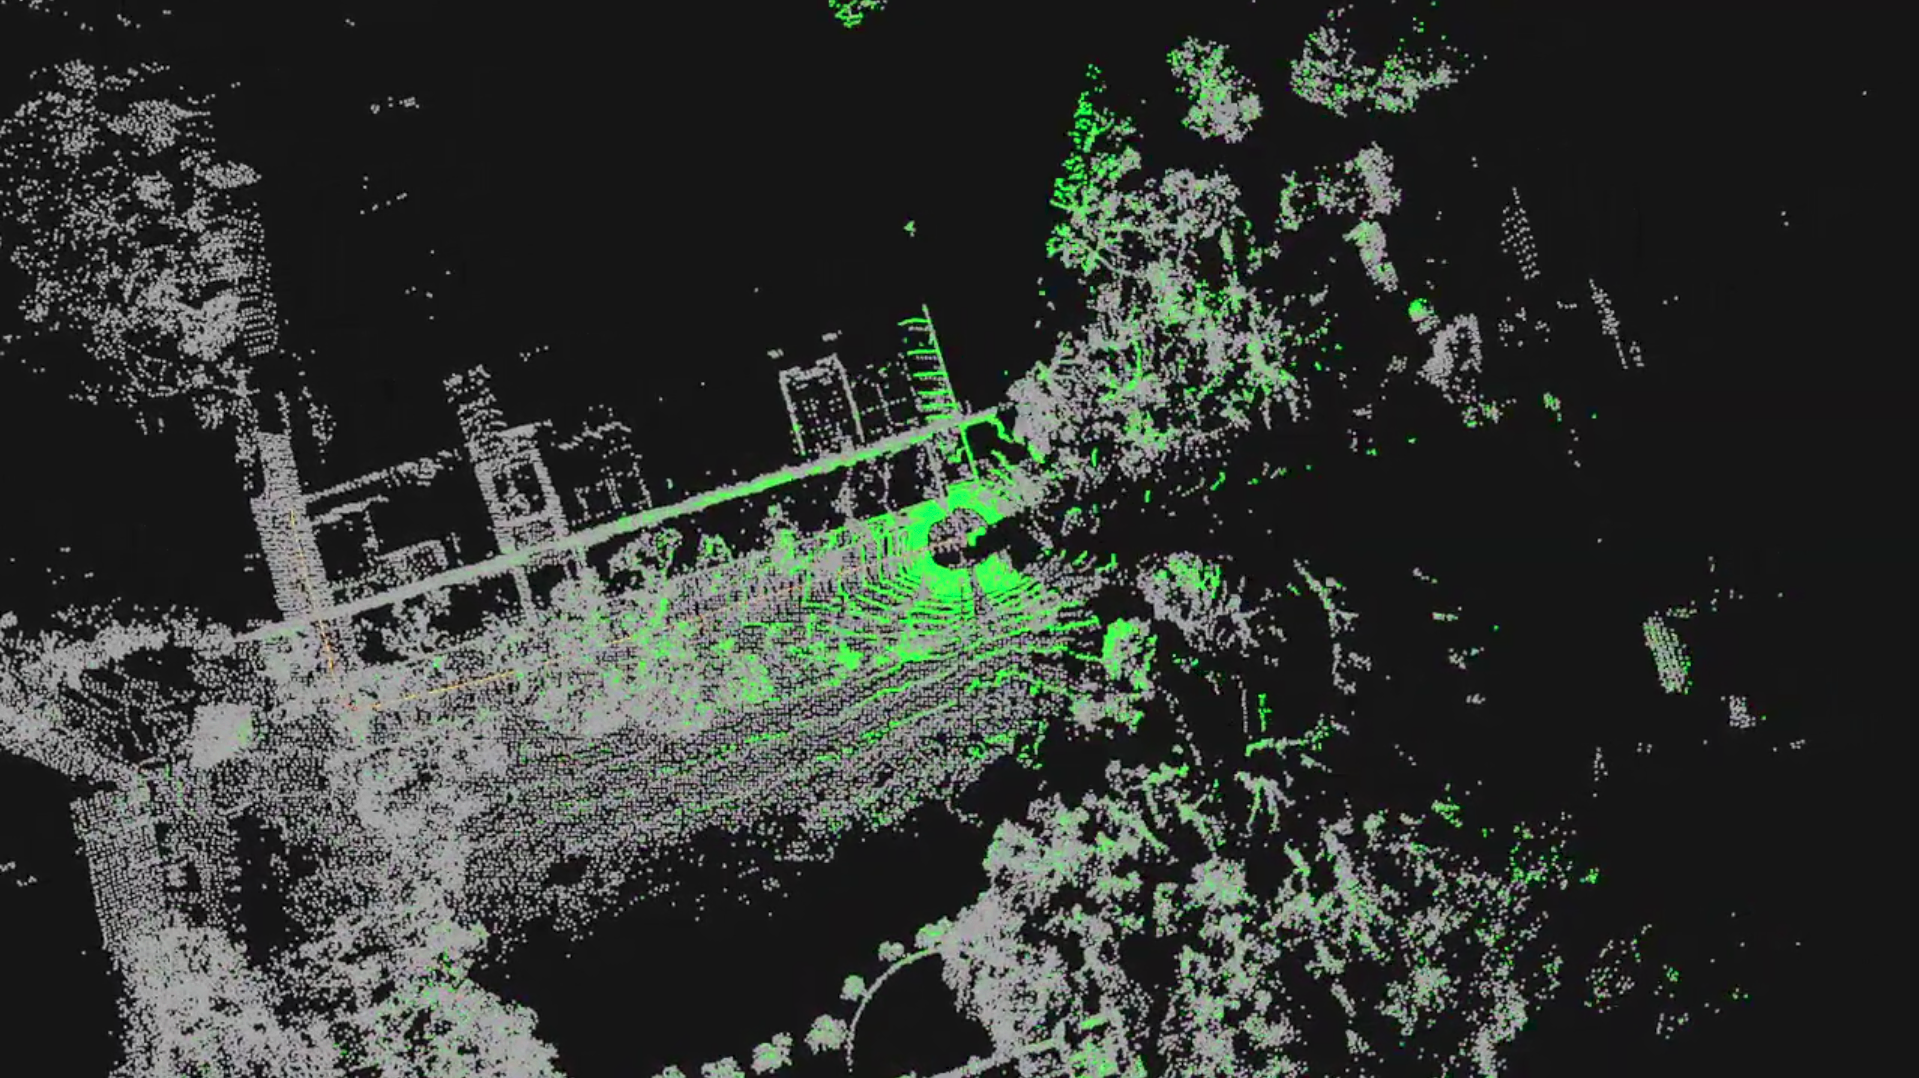
\includegraphics[width=\textwidth]{slam-1.png}
    \end{minipage}%
    \hfill
    \begin{minipage}{0.48\textwidth}
        \centering
        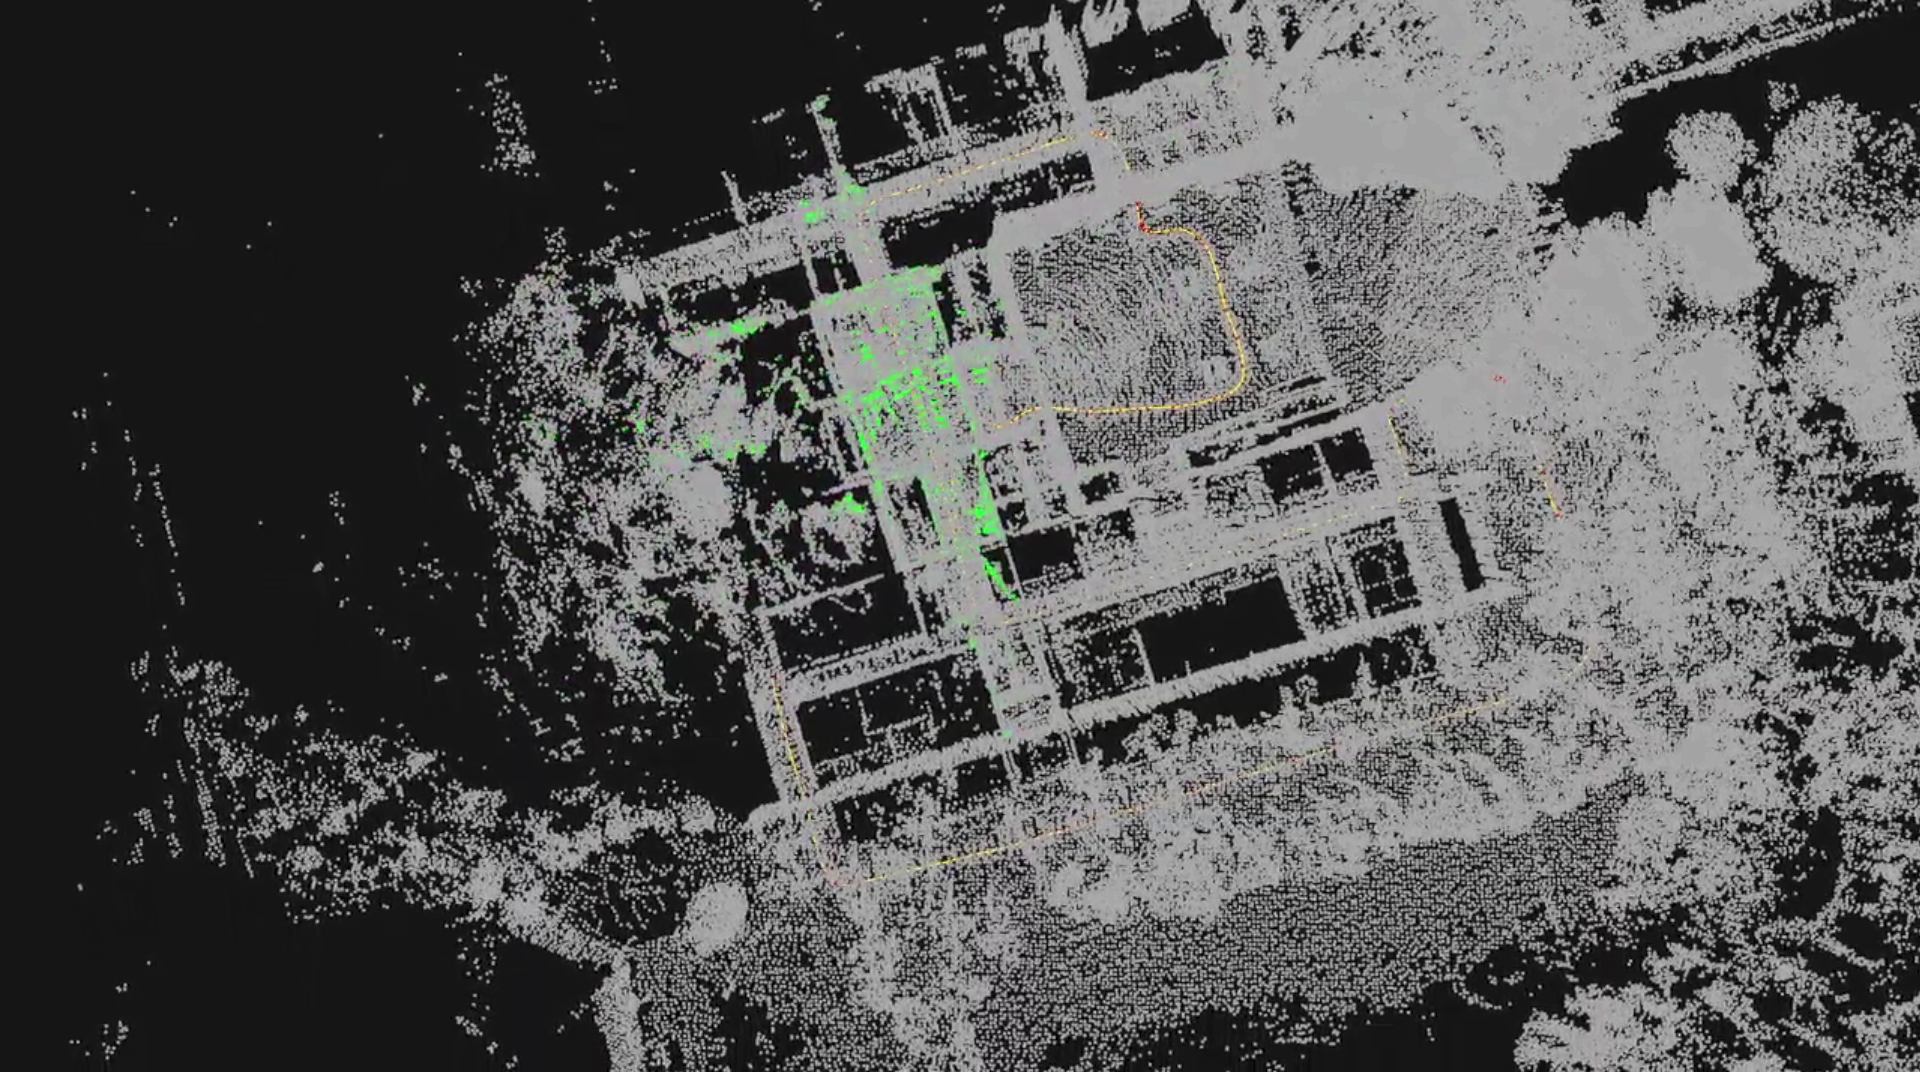
\includegraphics[width=\textwidth]{slam-2.png}
    \end{minipage}
    \caption{Globally optimized SLAM trajectory maps illustrating drift correction via loop closure constraints.}
    \label{fig:slam_result}
\end{figure}

\begin{figure}[H]
    \centering
    \begin{minipage}{0.31\textwidth}
        \centering
        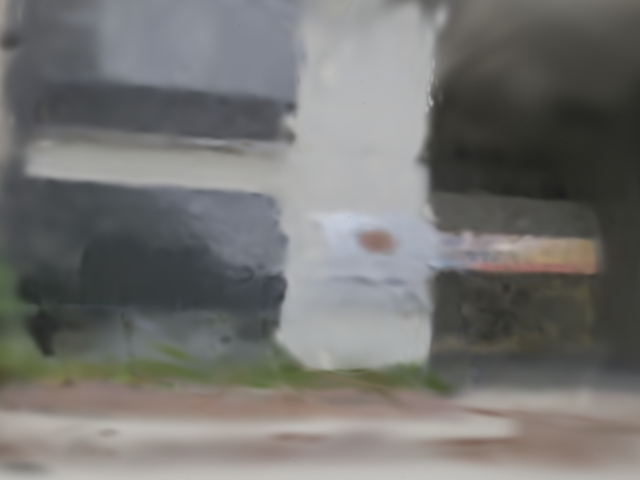
\includegraphics[width=\textwidth]{track1-1.png}
    \end{minipage}%
    \hfill
    \begin{minipage}{0.31\textwidth}
        \centering
        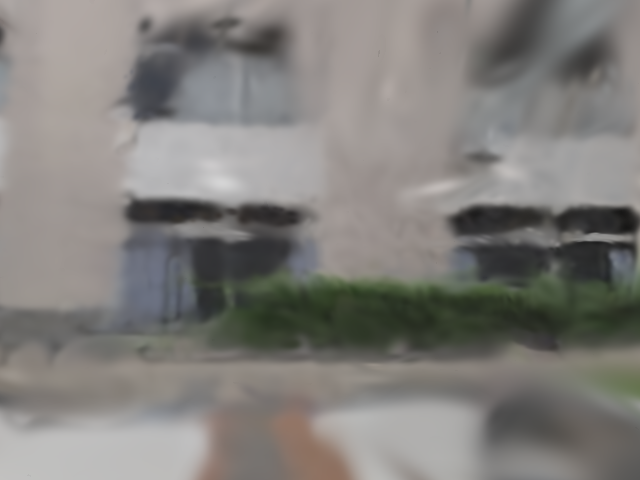
\includegraphics[width=\textwidth]{track1-2.png}
    \end{minipage}%
    \hfill
    \begin{minipage}{0.31\textwidth}
        \centering
        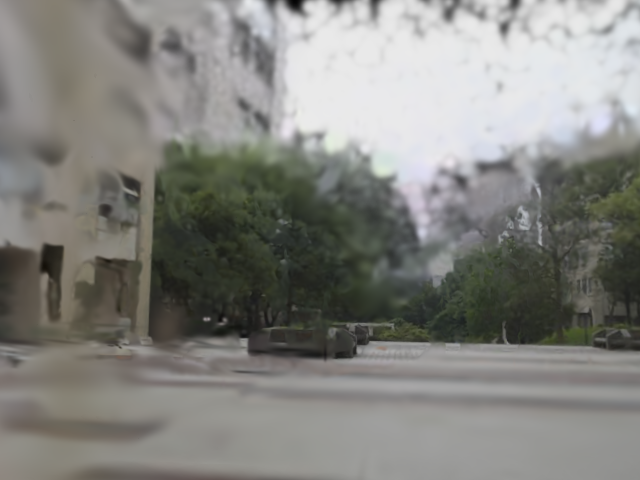
\includegraphics[width=\textwidth]{track1-3.png}
    \end{minipage}
    \caption{Visual reconstruction comparisons demonstrating 3DGS rendering fidelity for Track 1 novel viewpoints.}
    \label{fig:3dgs_track1}
\end{figure}

\begin{figure}[H]
    \centering
    \begin{minipage}{0.31\textwidth}
        \centering
        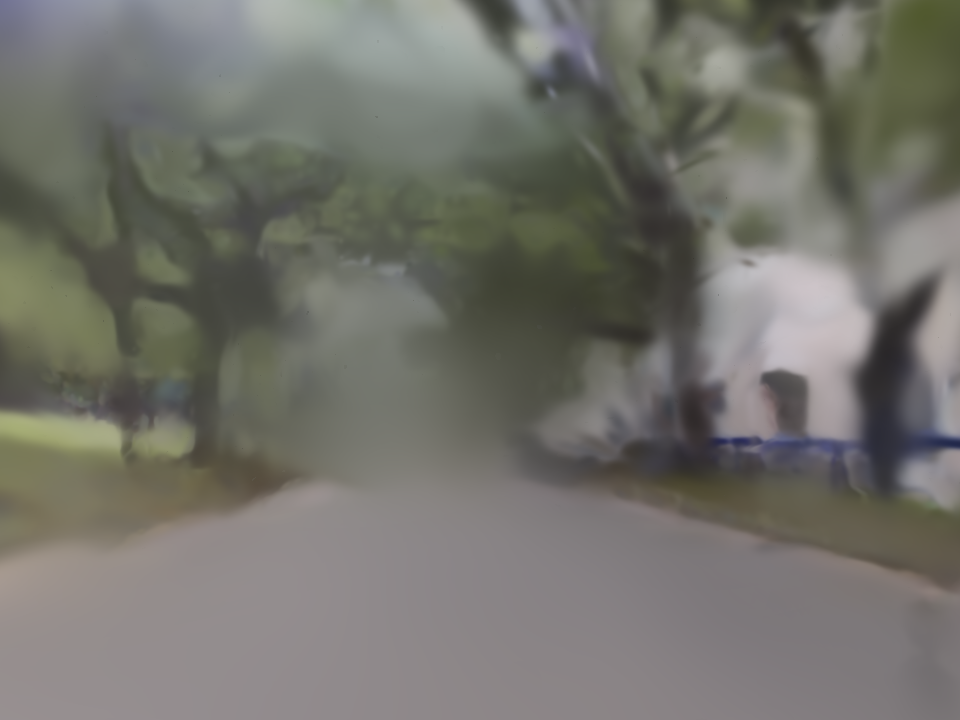
\includegraphics[width=\textwidth]{track3-1.png}
    \end{minipage}%
    \hfill
    \begin{minipage}{0.31\textwidth}
        \centering
        
\includegraphics[width=\textwidth]{track3-2.png}
    \end{minipage}%
    \hfill
    \begin{minipage}{0.31\textwidth}
        \centering
        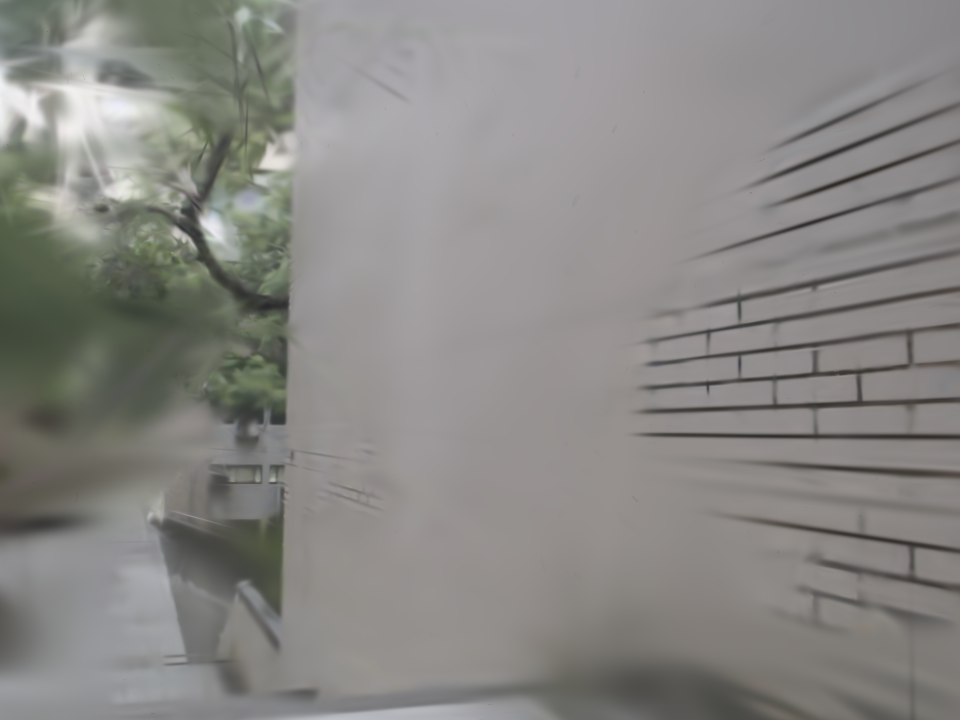
\includegraphics[width=\textwidth]{track3-3.png}
    \end{minipage}
    \caption{Visual reconstruction comparisons demonstrating 3DGS rendering fidelity for Track 3 novel viewpoints.}
    \label{fig:3dgs_track3}
\end{figure}

\section{Extra Experiment: Direct Image Interpolation Baseline}
We conducted an additional experiment implementing a baseline approach that directly interpolates adjacent training frames in 2D image-space to synthesize intermediate views along the vehicle's trajectory.

\begin{figure}[H]
    \centering
    \begin{minipage}{0.48\textwidth}
        \centering
        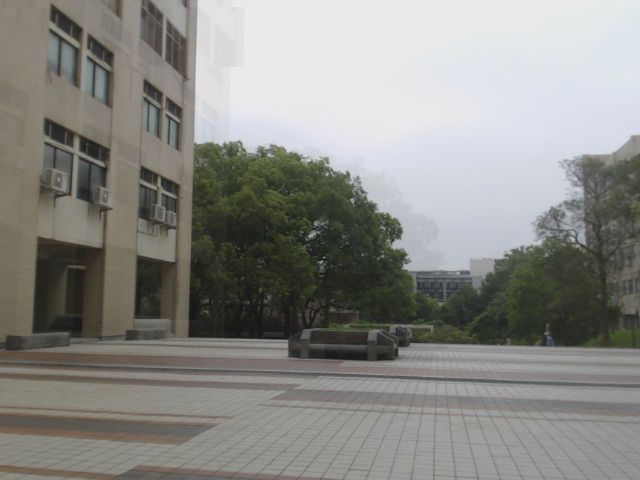
\includegraphics[width=\textwidth]{interpolation-1.png}
    \end{minipage}%
    \hfill
    \begin{minipage}{0.48\textwidth}
        \centering
        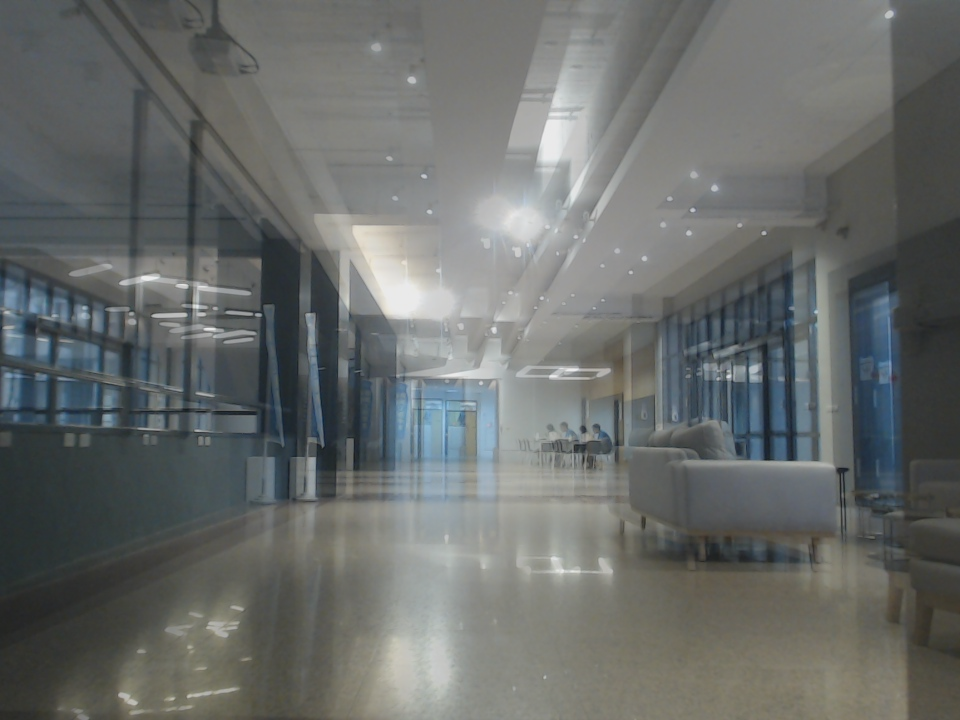
\includegraphics[width=\textwidth]{interpolation-2.png}
    \end{minipage}

    \vspace{0.04\textwidth}

    \begin{minipage}{0.48\textwidth}
        \centering
        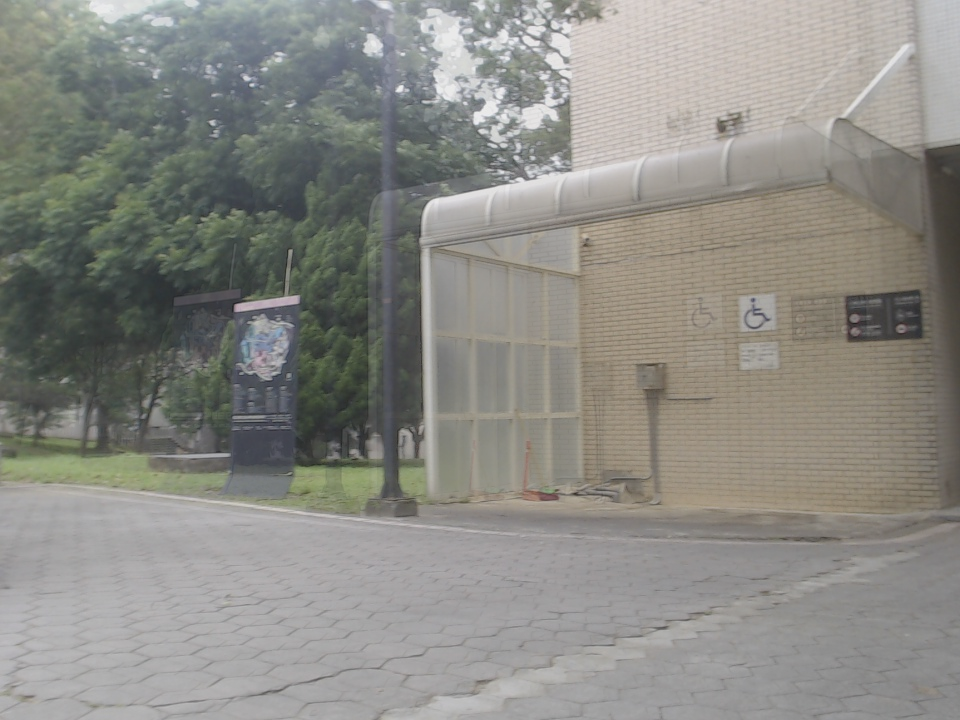
\includegraphics[width=\textwidth]{interpolation-3.png}
    \end{minipage}%
    \hfill
    \begin{minipage}{0.48\textwidth}
        \centering
        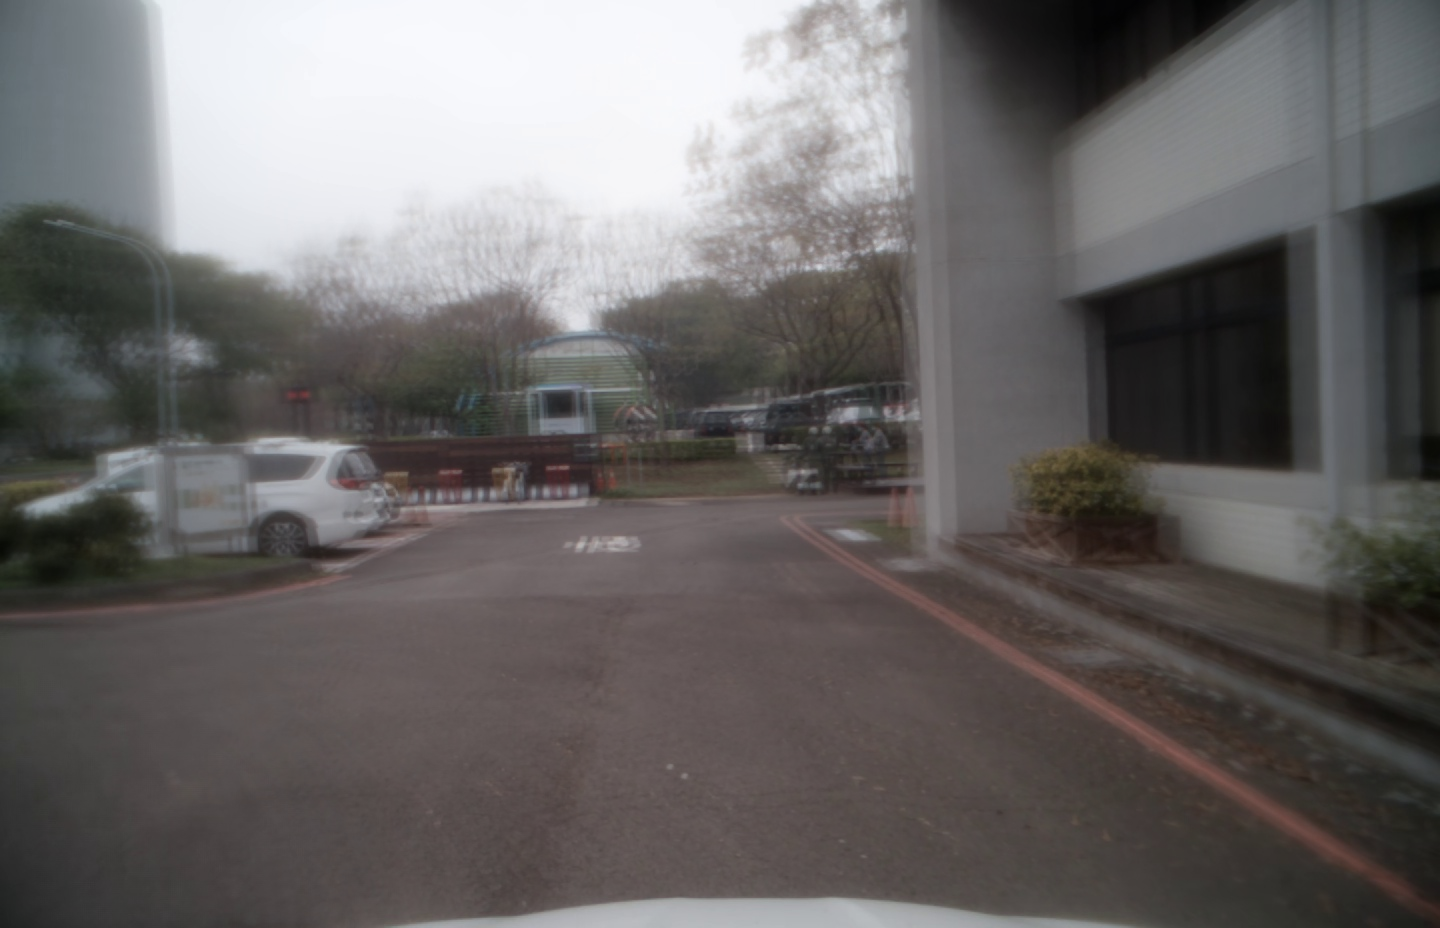
\includegraphics[width=\textwidth]{interpolation-4.png}
    \end{minipage}

    \vspace{0.04\textwidth}

    \begin{minipage}{0.48\textwidth}
        \centering
        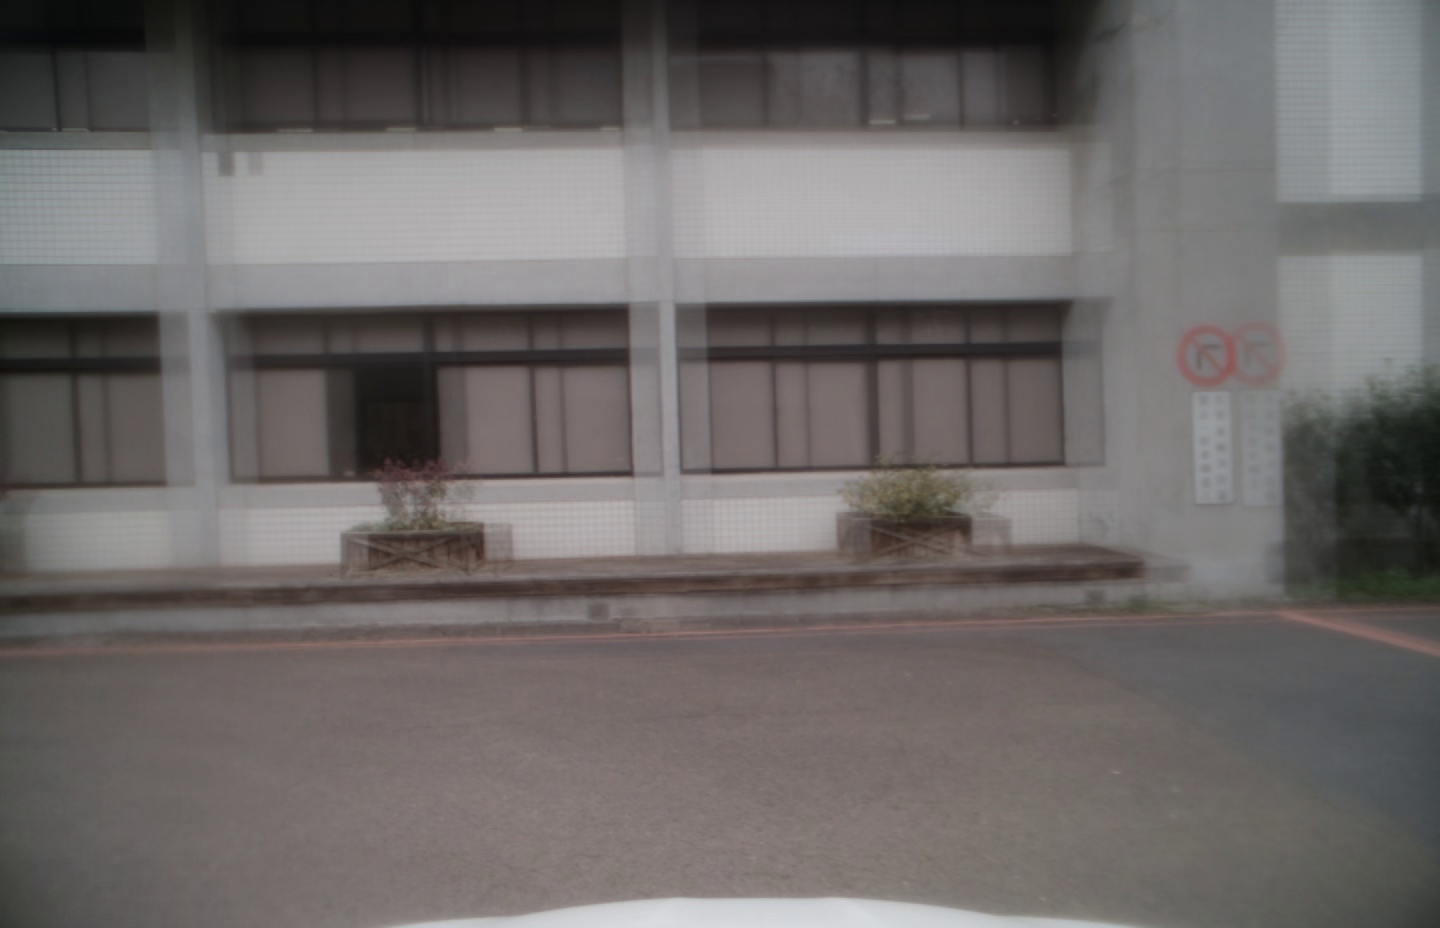
\includegraphics[width=\textwidth]{interpolation-5.png}
    \end{minipage}%
    \hfill
    \begin{minipage}{0.48\textwidth}
        \centering
        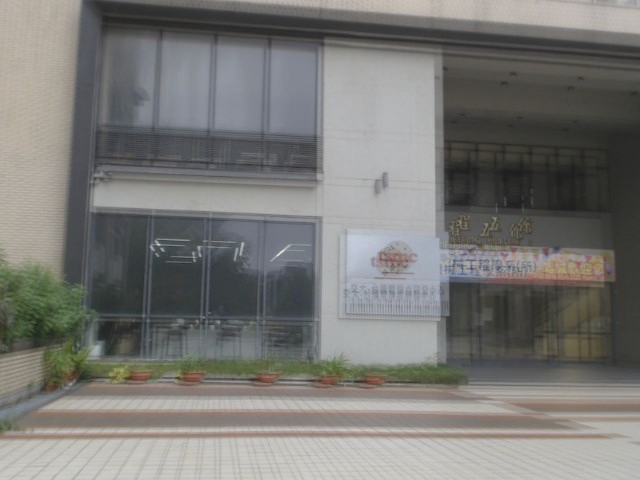
\includegraphics[width=\textwidth]{interpolation-6.png}
    \end{minipage}
    \caption{Evaluation metrics showing high structural similarity scores for the image-space interpolation baseline within dense training sequences.}
    \label{fig:interpolation_result}
\end{figure}

Although this interpolation baseline achieves high scores under dense frame constraints, it possesses fundamental limitations that make it unsuitable for autonomous driving applications:
\begin{itemize}
    \item \textbf{Lack of 3D Structure:} The method operates purely within the 2D pixel domain and does not build underlying 3D geometric primitives, rendering it incapable of generating spatial point cloud representations or physical maps.
    \item \textbf{Geometric Inconsistency:} It fails to maintain multi-view consistency when rendering from novel trajectories that deviate from the original training baseline path, producing severe ghosting and perspective distortion.
\end{itemize}

\section{Others}

To faithfully capture complex non-Lambertian materials, our system implements high-degree Spherical Harmonics $l_{max}=3$, allowing the ellipsoids to dynamically adjust their radiance based on the viewing angle $\mathbf{d}$. This enhancement enables the realistic reconstruction of view-dependent phenomena, such as specular glints on vehicle bodies and glass reflections. Additionally, a temporal cooldown gate is enforced within the loop closure thread to prevent redundant optimization overhead from sequentially triggered matches.

\end{document}
